\section{Brief introduction to AI}

\begin{frame}{What is AI?}
    % trình bày về 4 dạng AI, được định nghĩa trong quá khứ
    % nhấn mạnh về acting rationally
    % ai trong tương quan với ML và DL
\end{frame}

\begin{frame}{Foundation of AI}
    % có nhiều nền tảng:
    %     triết học (suy luận là gì?)
    %     kinh tế (nên quyết định như thế nào để tối đa lợi ích)
    %     toán học (làm sao biểu diễn suy luận?)
    %     khoa học thần kinh (não xử lý thông tin như nào?)
    %     ngôn ngữ (ngôn ngữ và suy nghĩ có liên quan gì?)
    %     ...
    % nhấn mạnh vào toán
\end{frame}

\subsection{History of AI}

\begin{frame}{History of AI}
    \begin{itemize}
        \item Summarize key milestones in AI's development
    \end{itemize}

    \begin{figure}
        \centering
        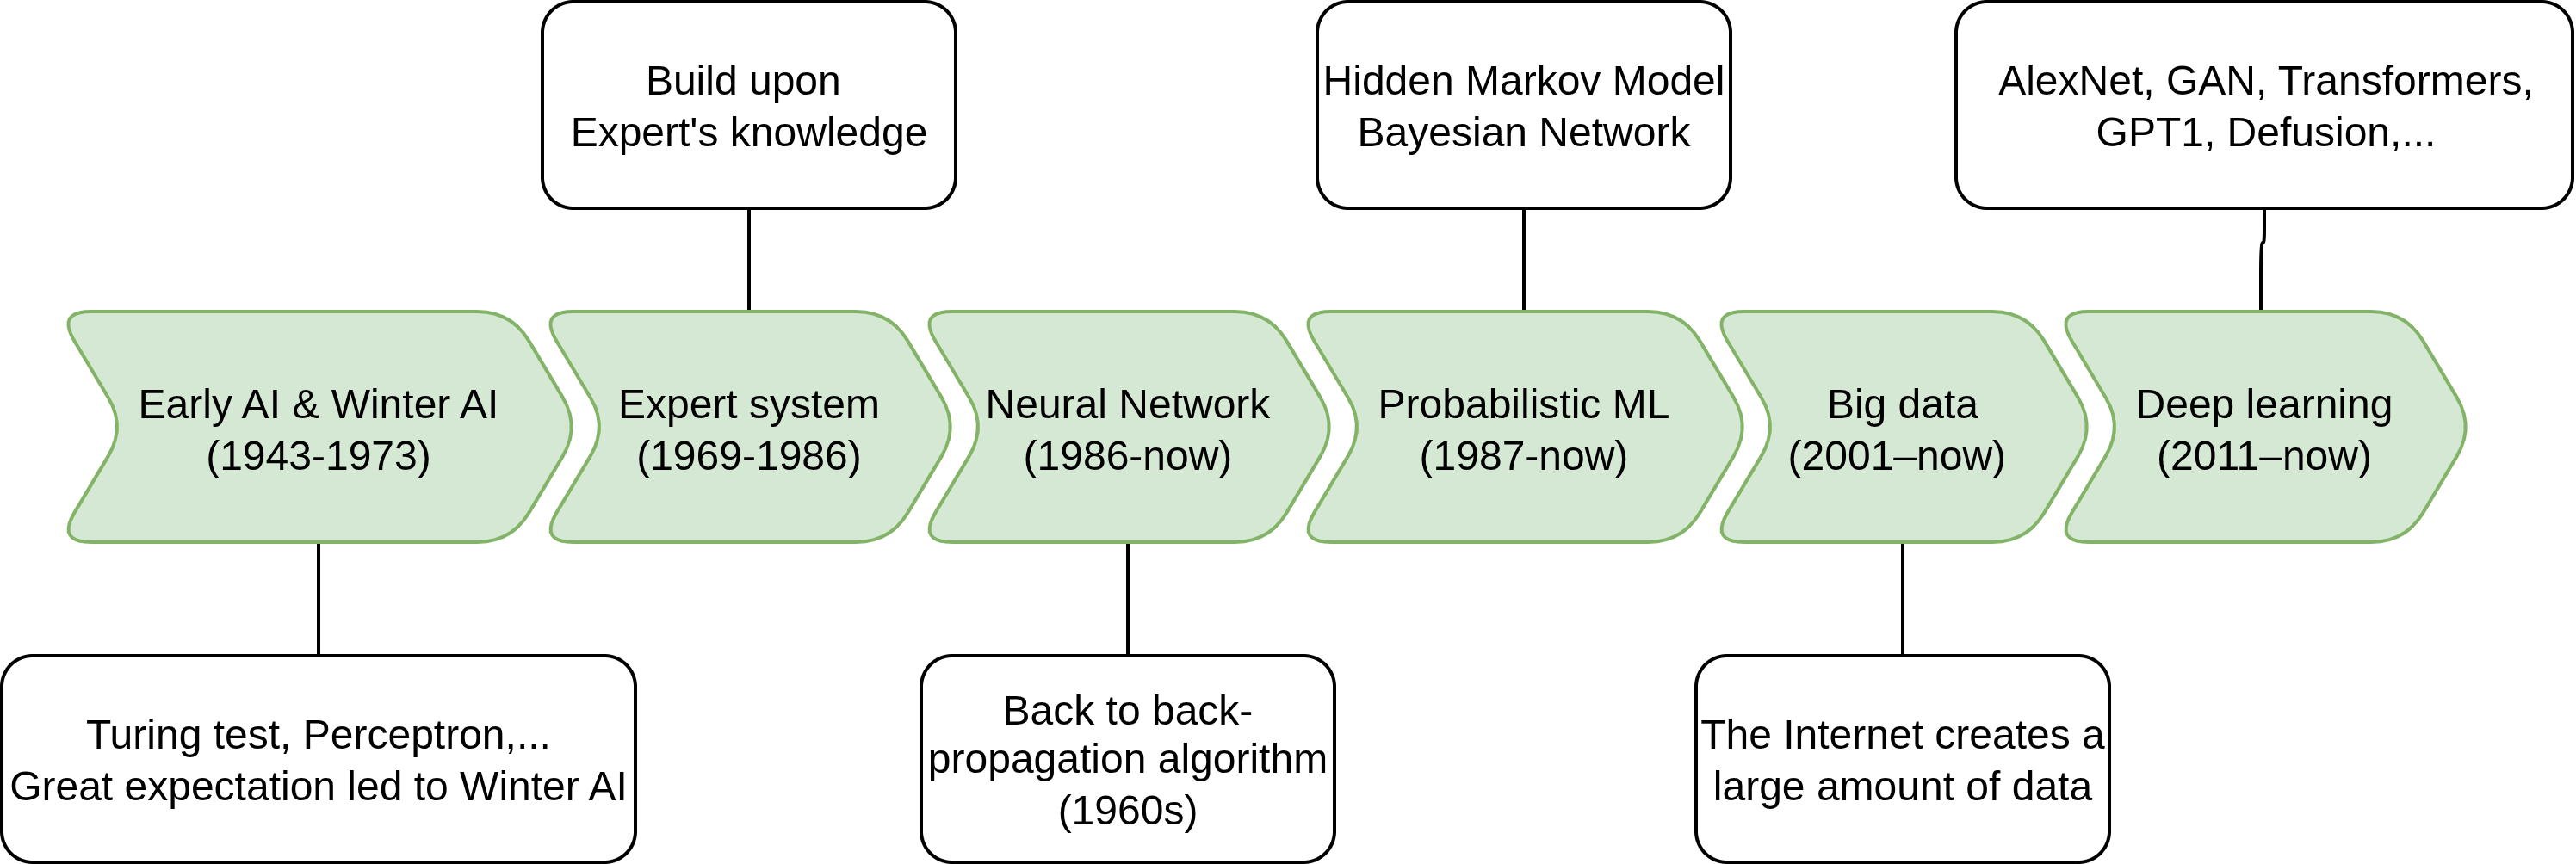
\includegraphics[width=\linewidth]{img/history_ai.png}
        \caption{Brief history of AI}
    \end{figure}
\end{frame}

\begin{frame}{From the Inception of AI to Winter AI (1943 - 1973)}
    % The inception of artificial intelligence (1943-1956)
    %     Alan Turing introduced Turing test, machine learning, generic algo, reinforcement learning
    %     Dartmouth workshop: John McCarthy gathered researcher and announced about AI
    \begin{columns}
        \begin{column}{0.5\textwidth}
            \begin{itemize}
                \item Turing test (1950) - An AI should act humanly (nowadays, ChatGPT can surpass the test!)
            \end{itemize}
        \end{column}

        \begin{column}{0.5\textwidth}
            \begin{figure}
                \centering
                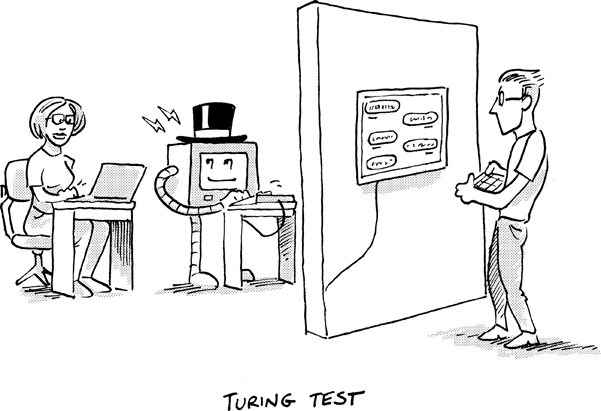
\includegraphics[width=\linewidth]{img/turing_test.png}
                \caption{One has to distinguish human and computer based on their output}
            \end{figure}
        \end{column}
    \end{columns}
\end{frame}

\begin{frame}{From the Inception of AI to Winter AI (1943 - 1973)}
    % Early enthusiasm (1952-1969):
    %     General problem solver: giải bài toán tìm đường (problem được mô hình hóa thành graph). idea kiểu như A* nhưng gà hơn
    %     John McCarthy proposed LIPS: xử lý suy luận logic, nhưng phải tự định nghĩa các thuật giải trong suy luận
    %     Perceptron (1962): a network can be modified so it can map any kinds of input-output (given the relationship between input and output)
    \begin{columns}
        \begin{column}{0.5\textwidth}
            \begin{itemize}
                \item Perceptron (1962) - The learning algorithm can train a perceptron to match (if existed) any input data
                \item Sadly, nones cared
            \end{itemize}
        \end{column}

        \begin{column}{0.5\textwidth}
            \begin{figure}
                \centering
                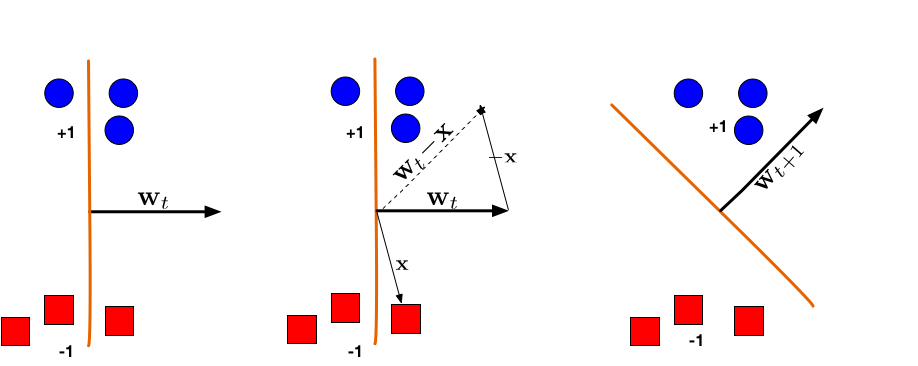
\includegraphics[width=\linewidth]{img/perceptron_update.png}
                \caption{If a data set is linearly separable, the Perceptron will find a separating hyperplane in a finite number of updates}
                % hình dung rằng: nếu chúng ta biểu diễn được chó và mèo lên hệ tọa độ (2 con này chắc chắn khác nhau) thì chúng ta có thể kẻ được một đường thẳng, phân biệt 2 con này --> biết đâu là chó, đâu là mèo
                % source: https://www.cs.cornell.edu/courses/cs4780/2018fa/lectures/lecturenote03.html
            \end{figure}
        \end{column}
    \end{columns}
\end{frame}

\begin{frame}{From the Inception of AI to Winter AI (1943 - 1973)}
    % Winter of AI (1966-1973)
    %     machine tried to imitate human (e^1.5=?) --> fail to perform well
    %     people thought that problems (which AI was trying to solve) is easy. most approaches were brute-force

    The failure of AI:
    \begin{itemize}
        \item Problem-solving systems worked by trial-and-error (brute-force) $\to$ Combinatorial explosion
        \item Designing AI temped to imitate human (e.g., A*, General problem solver,...)
    \end{itemize}

    \begin{figure}
        \centering
        \begin{subfigure}[b]{0.25\textwidth}            
            \centering
            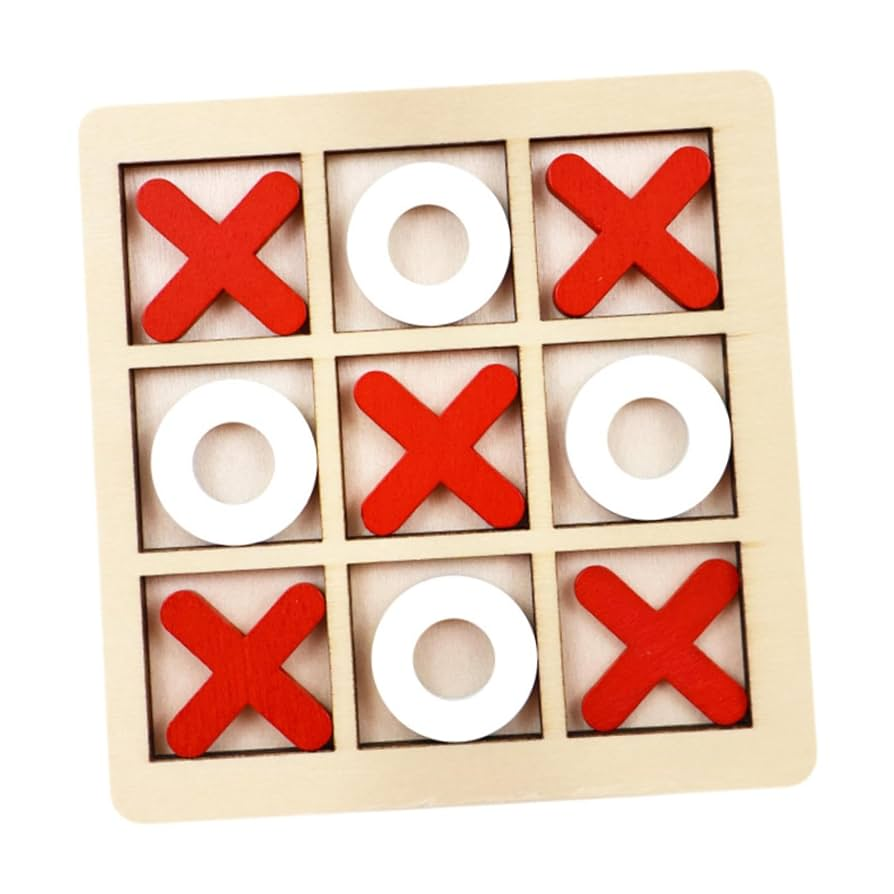
\includegraphics[width=\textwidth]{img/tic_tac_toe.png}
            \caption{Tic-Tac-Toe}
        \end{subfigure}%
        %
        %
        \begin{subfigure}[b]{0.25\textwidth}
            \centering
            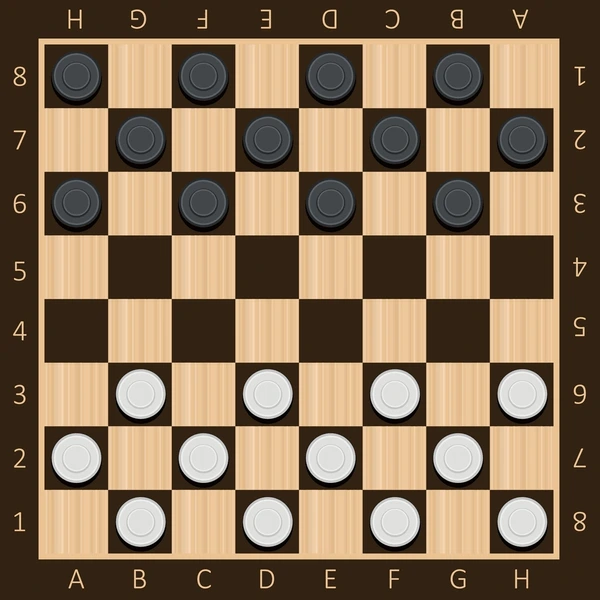
\includegraphics[width=\textwidth]{img/checker.png}
            \caption{Checker}
        \end{subfigure}
        \caption{These games can be solved by Search algorithm. Yet other games such as chess, go?}
    \end{figure}
\end{frame}

\begin{frame}{Expert system (1969 - 1986)}
    % Expert system  (1969-1986): chuyên gia nhập knowledge vào cho hệ thống. không khám phá luật tự động (apriori) và phụ thuộc chuyên gia

    An Expert system includes:
    \begin{itemize}
        \item A knowledge base (KB), which is a list of fact (e.g., All men are mortal; Socrates is a man)
        \item An inference engine, which takes the input and infer the output based on KB (e.g., Input: Is Socrates mortal?; Output: True)
        \item Prolog is a language supporting that inference
    \end{itemize}
\end{frame}

\begin{frame}{From Neural network to Deep learning (1986 - now)}
    % The return of neural networks (1986-present)
    %     Reinvented the back-propagation learning algorithm first developed in the early 1960s
    \begin{columns}
        \begin{column}{0.5\textwidth}
            \begin{itemize}
                \item Neural network: Back to back-propagation algorithm (1960s), which is used in many learning problems
                \item Probabilistic ML (1987): Hidden Markov model, Bayesian network % HMM can be used in speech recognition
                \item Massive of data is generated via the Internet (2001) $\to$ the need of data management
            \end{itemize}
        \end{column}

        \begin{column}{0.5\textwidth}
            \begin{figure}
                \centering
                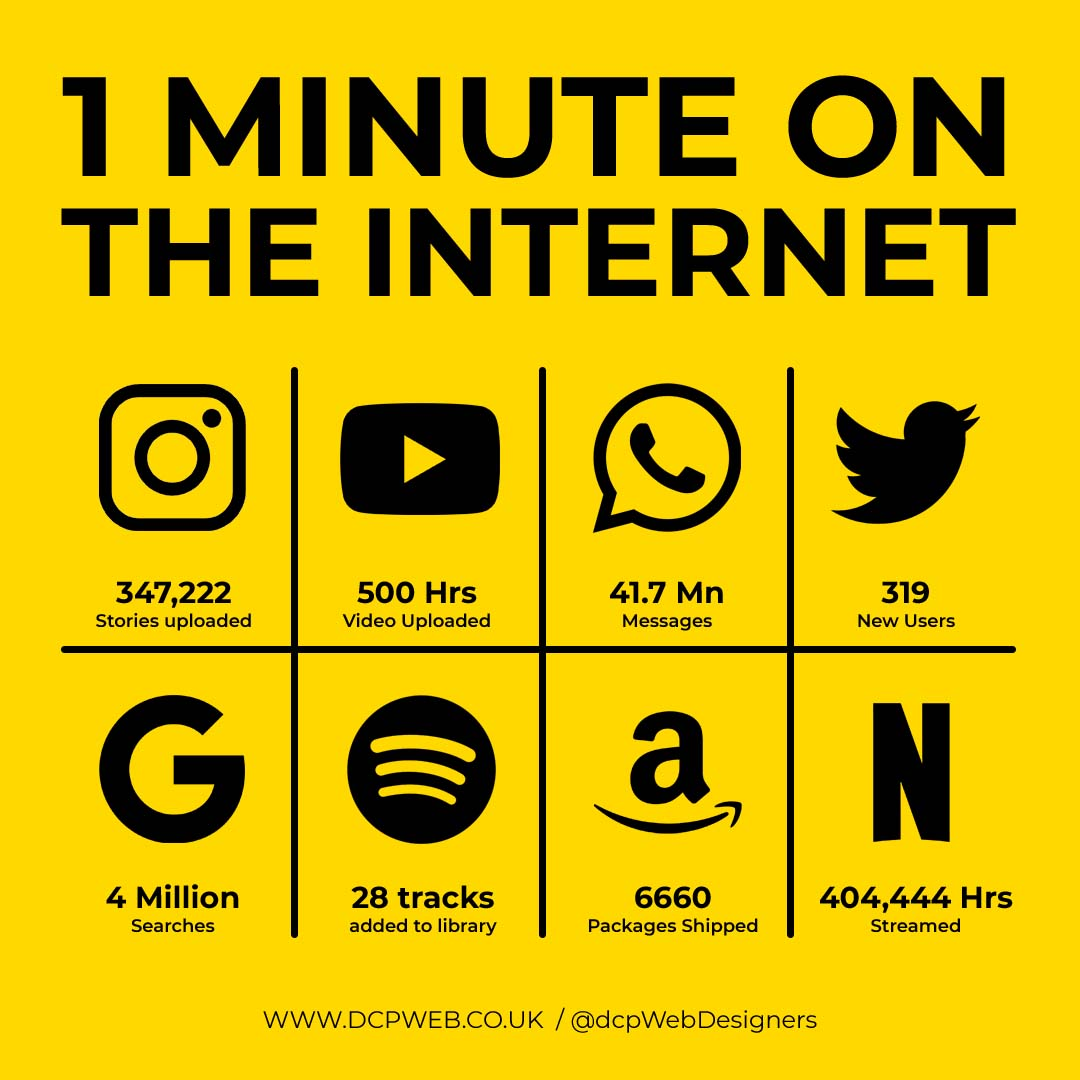
\includegraphics[width=0.8\linewidth]{img/statistic.png}
                \caption{Data generated in 1 minute}
            \end{figure}
        \end{column}
    \end{columns}
\end{frame}

\begin{frame}{From Neural network to Deep learning (1986 - now)}
    % big data (2001 - now)
    %     the creation of the internet facilities the creation of very large datasets

    \begin{columns}
        \begin{column}{0.5\textwidth}
            \alert{Many datasets appeared}
            \begin{itemize}
                \item ImageNet for vision models
                \item BookCorpus (4.5GB, ~7000 unpublished books) for GPT-1
                \item WebText (40GB text from Reddit) for GPT-2
                \item ...
            \end{itemize}
        \end{column}

        \begin{column}{0.5\textwidth}
            \begin{figure}
                \centering
                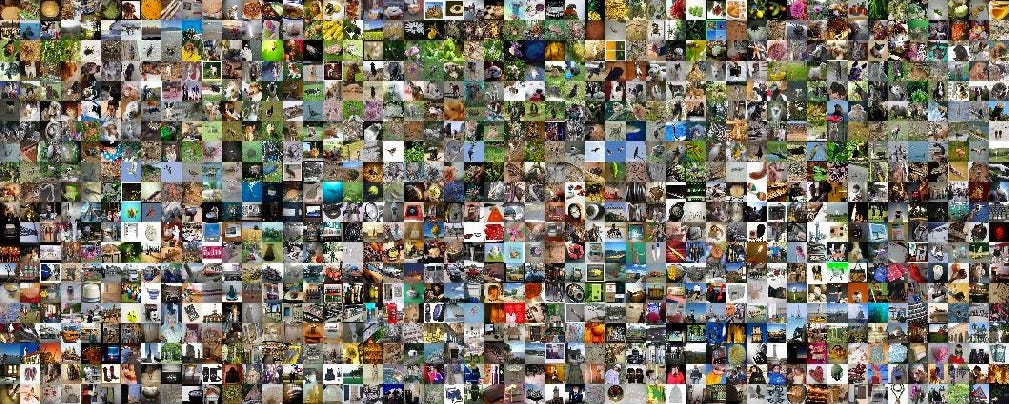
\includegraphics[width=\linewidth]{img/imagenet.png}
                \caption{ImageNet dataset: ~14m images, ~21k labels}
            \end{figure}
        \end{column}
    \end{columns}
\end{frame}

\begin{frame}{From Neural network to Deep learning (1986 - now)}
    % deep learning (2011 - now)
    %     ImageNet, AlexNet, GAN, Transformers, GPT,...

    \begin{columns}
        \begin{column}{0.6\textwidth}
            \alert{The development of processor} (CPU, GPU) leads to many successes:
            \begin{itemize}
                \item In 1997, Deep Blue (IBM) defeated World Chess Champion (algorithm: MinMax Search, Alpha-Beta pruning)
                \item In 2016, AlphaGo (Google) defeated World Go Champion (algorithm: Reinforcement learning, self-play)
                % \item In 2017, AlphaZero (Google) defeated AlphaGo and won in chess, shogi, go,...
                \item In 2017, \alert{Transformers} was proposed, opening a new chapter for AI: Large language model, new vision model, generative AI, agent,...
            \end{itemize}
        \end{column}

        \begin{column}{0.4\textwidth}
            \begin{figure}
                \centering
                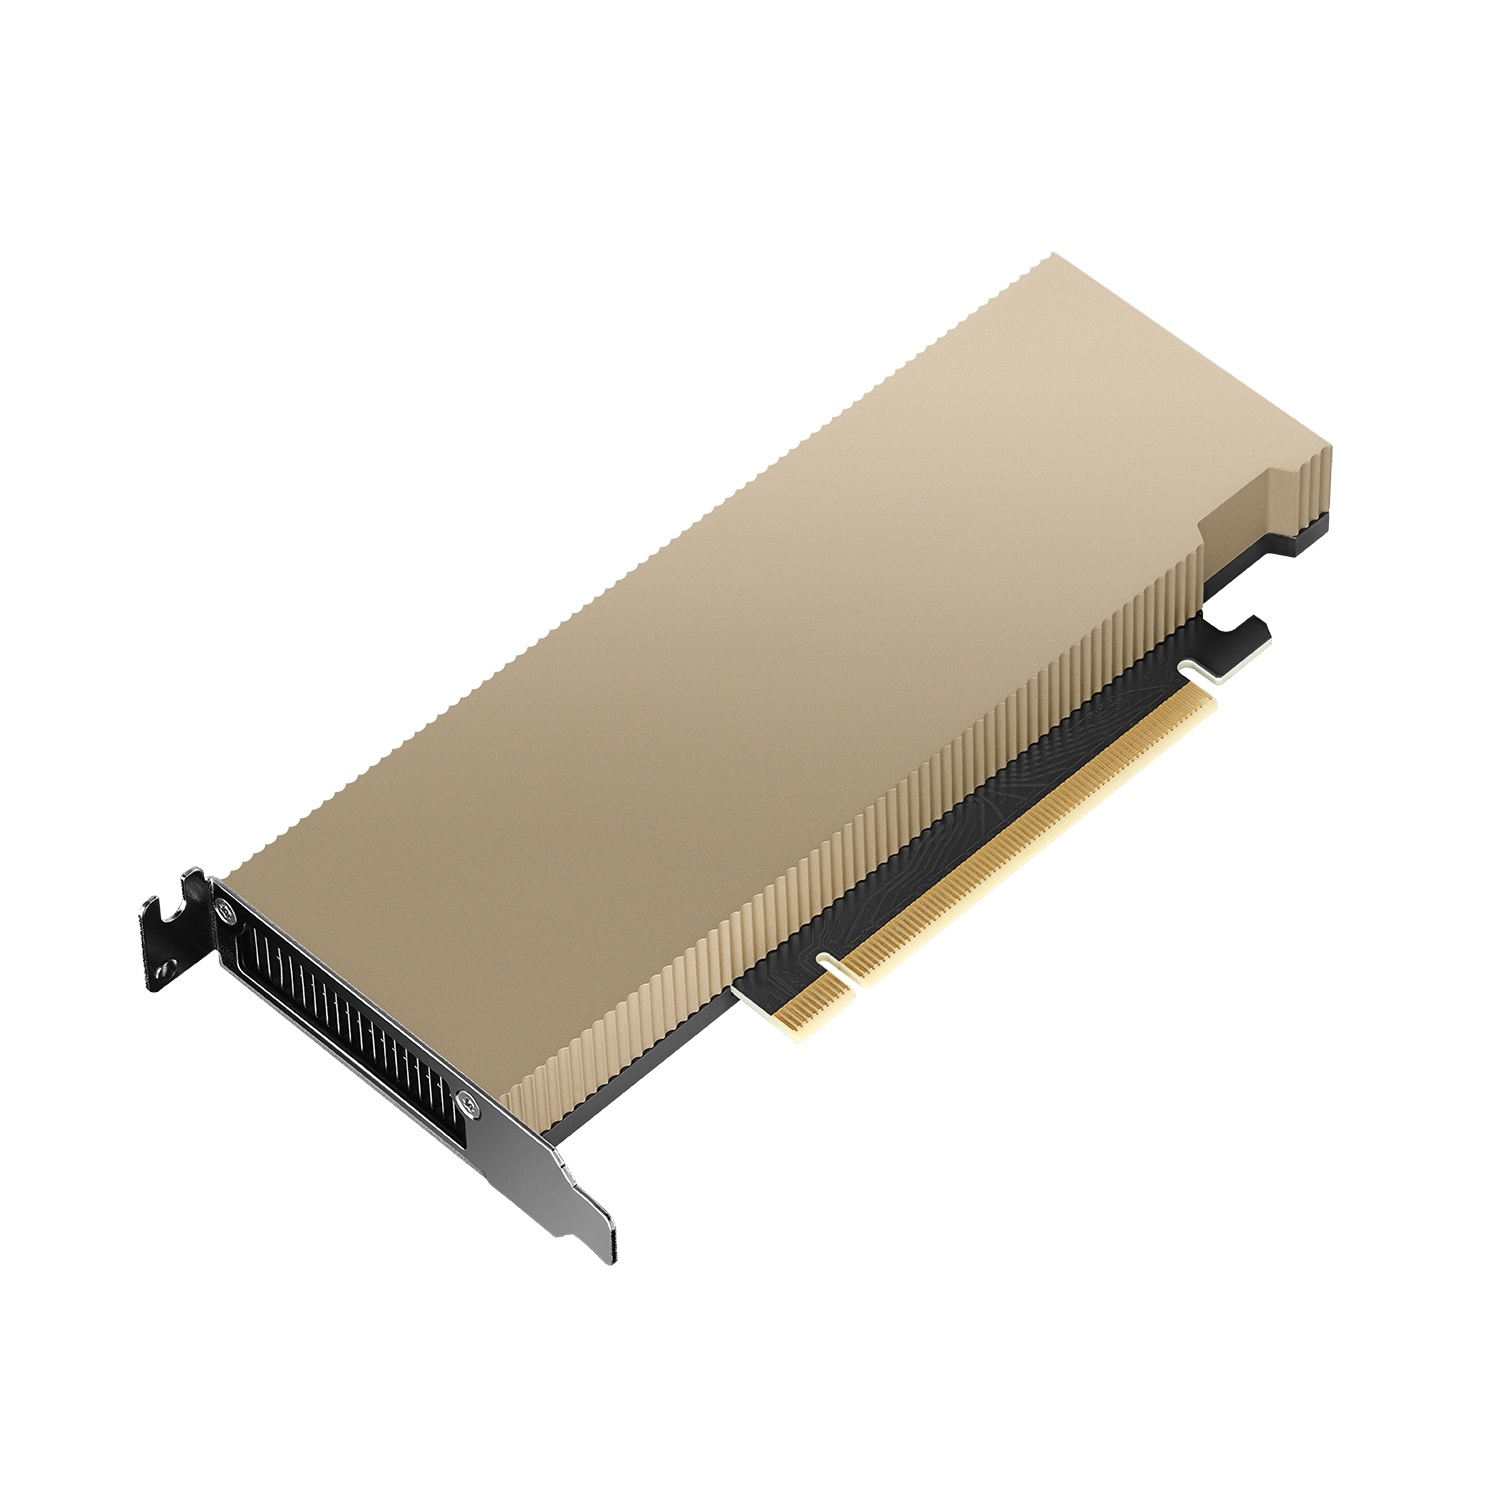
\includegraphics[width=0.8\linewidth]{img/nvidia_a100.png}
                \caption{Nvidia A100, 80GB, 6912 cores. 19.5 TFLOPS for the precision of FP64 Tensor core}
                % thực hiện 19.5*10^12 flops ~ 19.5 nghìn tỷ phép tính với độ chính xác 64bit (thực hiện trên ma trận)
            \end{figure}
        \end{column}
    \end{columns}
\end{frame}

\subsection{AI applications}

\begin{frame}{AI applications - Computer vision}
    
\end{frame}

\begin{frame}{AI applications - Natural language processing}
    
\end{frame}

\begin{frame}{AI applications - Robotic}
    
\end{frame}
